\section{PC-MTS Analyses: Supervision--Optimization Alignment}
\label{sec:pcmts-analysis}

This section is needed because the quality of a supervision target and its
value for subsequent policy optimization are different quantities.  PC-MTS is
designed for the latter: it keeps a target only when its score, component-wise
trade-off, local feasibility, and proximity to the frozen learner's rollout
support are jointly acceptable.  We first examine the observed
imitation-to-optimization reversal, and then specify the controls required to
separate policy compatibility from candidate count and training budget.

\subsection{The observed supervision--optimization reversal}
\label{sec:pcmts-mismatch}

Table~\ref{tab:supervision_mismatch} restates the reported comparison from the
main paper and makes the change induced by the common scalar-GRPO stage
explicit.  Score and Pareto selection produce the two strongest imitation
checkpoints (87.2 and 87.5 PDMS), yet both deteriorate under the subsequent
optimizer.  In contrast, PC-MTS deliberately gives up 0.3--0.6 imitation
points relative to those selectors and improves by 4.2 points after the same
optimization stage.  GT supervision also improves, but finishes 0.8 points
below PC-MTS.  Thus, ranking target sets by imitation PDMS would select Pareto,
whereas ranking them by optimized PDMS selects PC-MTS.  This reversal is the
direct evidence for the mismatch claimed in the paper.

\begin{table}[t]
\centering
\small
\caption{Supervision--optimization comparison on NAVSIM v1 under single-trajectory inference. All four rows are one paper-reported run; higher PDMS and GRPO change are better, and no variance is implied.}
\label{tab:supervision_mismatch}
\resizebox{\linewidth}{!}{%
\begin{tabular}{lccccc}
\toprule
method & il\_pdms & post\_scalar\_grpo\_pdms & grpo\_change\_points & evidence & runs \\
\midrule
GT & 86.4 & 90.3 & 3.9 & paper reported & 1 reported \\
Score & 87.2 & 85.8 & -1.4 & paper reported & 1 reported \\
Pareto & 87.5 & 86.7 & -0.8 & paper reported & 1 reported \\
PC-MTS & 86.9 & 91.1 & 4.2 & paper reported & 1 reported \\
\bottomrule
\end{tabular}%
}
\end{table}


\begin{figure}[t]
  \centering
  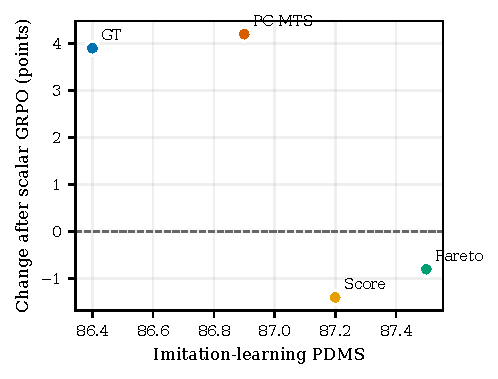
\includegraphics[width=\linewidth]{figures/generated/supervision_mismatch.pdf}
  \caption{Paper-reported imitation PDMS versus the change after the common
  scalar-GRPO stage on NAVSIM v1.  A high imitation score alone does not
  predict optimization value: Score and Pareto regress, whereas PC-MTS gains
  4.2 points.  Each marker is one reported point estimate; the paper does not
  state run/seed aggregation and no synthetic error bars are shown.}
  \label{fig:supervision-mismatch}
\end{figure}

The comparison should be interpreted at the level supported by the evidence.
It demonstrates that a higher-scoring imitation checkpoint need not be a
better starting distribution for GRPO, and that the PC-MTS set is compatible
with a large positive update in this run.  The archived paper table does not
contain scene-level outputs, acceptance counts, or multiple seeds for these
four cells.  Consequently, it does not by itself establish that the reversal
is invariant to seed, nor does it isolate candidate count from the four
filtering decisions.  We therefore do not attach synthetic error bars or
policy-distance values to these points.

\subsection{Candidate-count-matched reconstruction protocol}
\label{sec:pcmts-matched-protocol}

The released reproduction configuration turns the missing causal controls
into a predeclared, low-ambiguity experiment.  All four variants start from the
same GT-only checkpoint, use the same candidate sources, contribute exactly
one target per scene and update, train imitation learning for 200 epochs, and
then run scalar GRPO with 16 rollouts per scene for 10 epochs.  Within each
navigation-command/source stratum, accepted candidates are deterministically
subsampled to the smallest retained count across variants.  The non-GT
sampling probability is held fixed, so a method cannot receive more gradient
updates merely because it retains more candidates.  Empty strata fall back to
the logged trajectory.  In addition to final PDMS, a 300-update diagnostic
records the early GRPO gain before long-horizon training effects can dominate.

For a fully specified reconstruction when the original resolved PC-MTS
manifest is unavailable, the release marks the following as \emph{proposed
reproduction settings}, not measured settings of the reported run: a rollout
bank of 16, $K=3$ neighbors, a command-conditional 0.95 calibration quantile,
and eight temporally correlated local perturbations.  The rollout bank and
calibration queries are disjoint by construction.  Three predeclared training
seeds (20260726, 20260727, and 20260728) are used for the reconstruction, while
bootstrap seed 2027 is reserved for analysis and is never treated as an additional
training run.  These choices fill the executable configuration without
retroactively attributing unrecorded hyperparameters to the main-paper result.

For each run, the pipeline records retained candidates, acceptance rate,
candidate-source composition, feasible rollout rate, feasible high-quality
rate, all-infeasible-group rate, zero-score rate, the 10th percentile,
CVaR-10, 300-update gain, and final scalar-GRPO PDMS.  Method differences are
computed on identical scenes with a 10,000-resample paired bootstrap; means
and standard deviations are reported across the three training seeds.

\subsection{Filter attribution and sensitivity}
\label{sec:pcmts-components}

The component experiment is cumulative: (i) aggregate Score only, (ii) Score
plus the component-wise Pareto gate, (iii) the preceding gates plus calibrated
policy compatibility, and (iv) the full selector with local-feasibility
testing.  Counts are matched after each gate, rather than relaxing a stricter
gate to reach a target count.  This distinction matters: a matched count must
not reintroduce candidates that failed the mechanism being tested.  The
decisive diagnostic is not imitation PDMS alone, but whether adding a gate
raises feasible rollout density and converts the fixed-budget GRPO change from
negative to positive.

The companion sensitivity protocol varies one factor at a time: rollout-bank
size in $\{8,16,32\}$, $K$ in $\{1,3,5\}$, calibration quantile in
$\{0.90,0.95,0.975\}$, and perturbation count in $\{4,8,16\}$.  Compatibility
alternatives are compared at the same acceptance rate: candidate-to-GT
ADE/FDE, distance to the deterministic policy output, minimum rollout-bank
distance, average $K$-nearest distance, and command-calibrated $K$-nearest
distance.  These are evidence-bounded planned analyses: the release contains
their configurations and logging schema, but no unexecuted outcome is used to
support the paper's reported 91.1 PDMS.

Taken together, the existing reversal and the matched protocol close two
different parts of the argument.  The former establishes that isolated target
quality can disagree with downstream optimization value; the latter defines
the experiment needed to attribute that disagreement specifically to policy
compatibility rather than supervision quantity.
